%!Tex Root = ../Tutorat3.tex
% ./Packete.tex
% ./Design.tex
% ./Deklarationen.tex
% ./Aufgabe1.tex
% ./Aufgabe2.tex
% ./Aufgabe4.tex
% ./Aufgabe5.tex
% ./Bonus.tex

\section{Task 3}

\setcounter{task}{1}

\begin{frame}[shrink=10]{Task 3}{Earliest Deadline First}
  \vspace{0.5cm}
  \begin{tasknoinc}
    \centering
    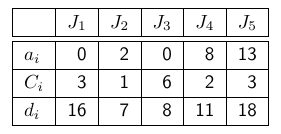
\includegraphics[height=0.2\paperheight]{./figures/3_tab.png}
  \end{tasknoinc}
  \begin{requirements}
    \begin{itemize}
      \item is \alert{preemptive}
      \item \alert{arbitrary arrival times}
      \item the tasks are \alert{independent}
      \item \alert{minimizes} the \alert{maximum lateness}
      \item $min(d_i)$ for all remaning tasks $J_i$  that have already \alert{arrived} (are ready) and \alert{not finished} \alert{every time} the \alert{arrival time} of a task is reached
    \end{itemize}
  \end{requirements}
\end{frame}

\begin{frame}{Task 3}{Earliest Deadline First}
  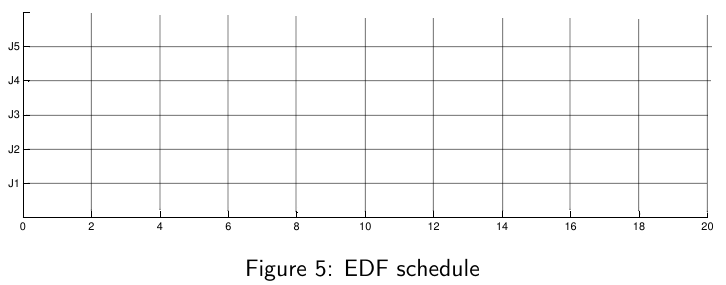
\includegraphics[width=\textwidth]{./figures/3_empty.png}
\end{frame}

\begin{frame}{Task 3}{Earliest Deadline First}
  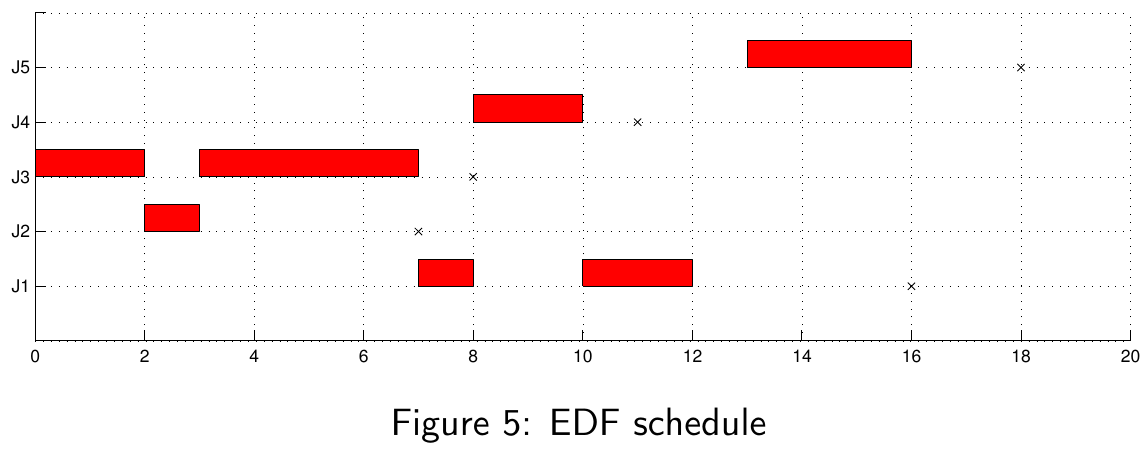
\includegraphics[width=\textwidth]{./figures/3_sol.png}
\end{frame}

\begin{frame}{Task 3}{Earliest Deadline First}
  \begin{tasknoinc}
    \begin{itemize}
      \item at time $t = 3$, a new task $J_x$ arrives with execution time $C_x = 2$ and deadline $d_x = 10$.
      \item still \alert{guarantee the schedulability} of task set?
    \end{itemize}
  \end{tasknoinc}
  \begin{requirements}
    \begin{itemize}
      \item \alert{acceptance test:} $\displaystyle \forall i=1, \ldots, n \quad t+\sum_{k=1}^i c_k(t) \leq d_i$
    \end{itemize}
  \end{requirements}
\end{frame}

\begin{frame}[allowframebreaks]{Task 3}{Earliest Deadline First\vspace{0.5cm}}
  \begin{itemize}
    \item \alert{check:} with $J_x$ schedule \alert{still feasible}
    \item compute \alert{ahead} the \alert{finishing times} in consideration of $J_x$
    \item consider the tasks \alert{in order of increasing deadlines:}
  \end{itemize}
  \begin{figure}
  \centering
  \begin{tabular}{|l|r|r|r|r|r|r|}
    \hline             & $J_2$ & $J_3$ & $J_X$ & $J_4$ & $J_1$ & $J_5$ \\
    \hline \hline$a_i$ & 2     & 0     & 3     & 8     & 0     & 13 \\
    \hline$C_i$        & 1     & 6     & 2     & 2     & 3     & 3 \\
    \hline$d_i$        & 7     & 8     & 10    & 11    & 16    & 18 \\
    \hline
  \end{tabular}
  \end{figure}
  \begin{itemize}
    % \item \alert{on-line scenario:} consider only tasks currently present in the system
    % \item test performed every time a new \alert{task arrives} [among \alert{all active task}]
    \item test performed every time a new \alert{task arrives} among \alert{all active task}
    % \item \alert{before} $J_x$ arrives at $t=3$ we have:
    % \begin{itemize}
    %   \item tasks $J_1$, $J_2$ and $J_3$ are feasible
    %   \item task $J_2$ finishes \alert{before} its \alert{deadline} at $t = 3$
    %   \item \alert{up to} $t = 3$ \alert{all} active tasks in the system are \alert{feasible}
    % \end{itemize}
  % \item at $t = 3$ we have [active tasks:] $\{J_1, J_3, J_x\}$
  \item at $t = 3$ we have active tasks: $\{J_1, J_3, J_x\}$
    \begin{itemize}
      % \item $f_0=t=3$
      \item $t=3$
      % \item Task $J_3: f_1=f_0+c_3(3)=3+4=7 \leq 8$ $\checkmark$
      % \item Task $J_3: f_1=t+c_3(3)=3+4=7 \leq 8$ $\checkmark$
      % \item Task $J_x: f_2=f_1+c_x(3)=7+2=9 \leq 10$ $\checkmark$
      % \item Task $J_1: f_3=f_2+c_1(3)=9+3=12 \leq 16$ $\checkmark$
      \item Task $J_3: f_1=t+c_3=3+4=7 \leq 8$ $\checkmark$
      \item Task $J_x: f_2=f_1+c_x=7+2=9 \leq 10$ $\checkmark$
      \item Task $J_1: f_3=f_2+c_1=9+3=12 \leq 16$ $\checkmark$
      \item Thus, at $t=3$ \alert{all} tasks in the system are feasible
    \end{itemize}
\item The next task to arrive is $J_4$. It arrives at $t=8$. At $t=8$, we have three active tasks: $\{J_x, J_4, J_1\}$
  \begin{itemize}
    % \item Put $f_0=t=8$
    \item Put $t=8$
    % \item Task $J_x: f_1=t+c_x(8)=8+1=9 \leq 10$ $\checkmark$
    % \item Task $J_4: f_2=f_1+c_4(8)=9+2=11 \leq 11$ $\checkmark$
    % \item Task $J_1: f_3=f_2+c_1(8)=11+3=14 \leq 16$ $\checkmark$
    \item Task $J_x: f_1=t+c_x=8+1=9 \leq 10$ $\checkmark$
    \item Task $J_4: f_2=f_1+c_4=9+2=11 \leq 11$ $\checkmark$
    \item Task $J_1: f_3=f_2+c_1=11+3=14 \leq 16$ $\checkmark$
    \item Thus, at $t=8$ \alert{all} tasks in the system are feasible.
  \end{itemize}
\item next task $J_5$ arrives at $t=13$. At $t=13$, we have two active tasks: $\{J_1, J_5\}$
    \begin{itemize}
      % \item Put $f_0=t=13$
      \item Put $t=13$
      % \item Task $J_1: f_1=t+c_1(13)=13+1=14 \leq 16$ $\checkmark$
      % \item Task $J_5: f_2=f_1+c_5(13)=14+3=17 \leq 18$ $\checkmark$
      \item Task $J_1: f_1=t+c_1=13+1=14 \leq 16$ $\checkmark$
      \item Task $J_5: f_2=f_1+c_5=14+3=17 \leq 18$ $\checkmark$
      \item hence, the whole \alert{schedule is feasible}
    \end{itemize}
  \end{itemize}
\end{frame}

\begin{frame}{Task 3}{Earliest Deadline First}
  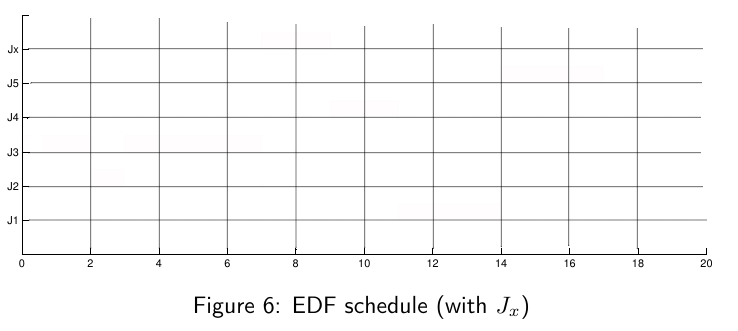
\includegraphics[width=\textwidth]{./figures/3_empty_2.png}
\end{frame}

\begin{frame}{Task 3}{Earliest Deadline First}
  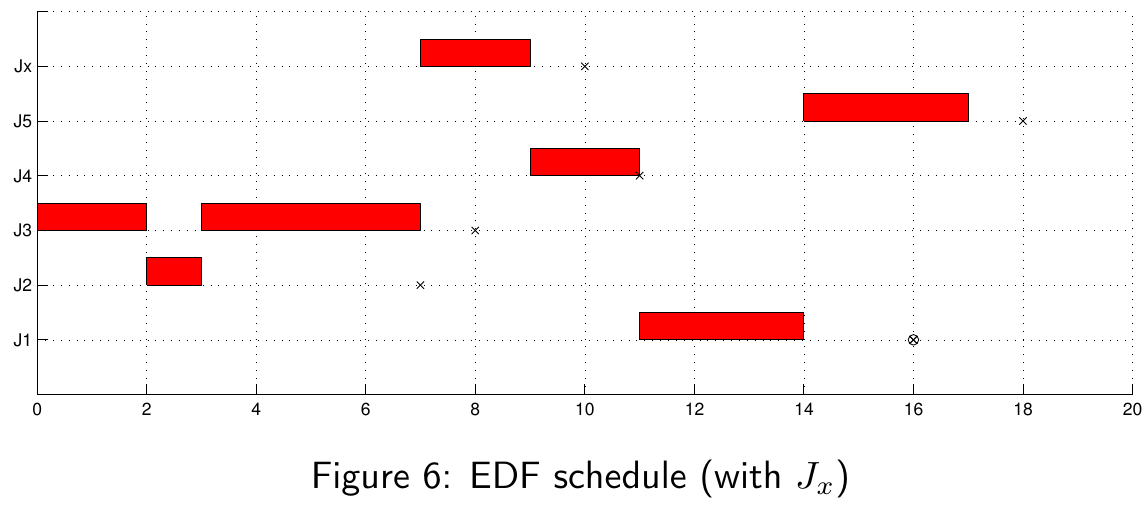
\includegraphics[width=\textwidth]{./figures/3_sol_2.png}
\end{frame}
